\documentclass[a4paper,12pt]{article}
\usepackage{xeCJK}          % 中文支持
\usepackage{fontspec}       % 英文/数学字体
\usepackage{amsmath, amssymb} % 数学公式
\usepackage{graphicx}       % 插入图片
\usepackage{hyperref}       % 目录超链接
\usepackage{geometry}       % 页面布局
\usepackage{bm}             % 粗体
\usepackage{xcolor}         % 颜色
\usepackage{tabularx}       % 表格环境
\usepackage{tikz}           % TikZ 绘制主对角线斜线
\usepackage{tcolorbox}
\usepackage{xstring}
\usepackage{pgfplots}
\pgfplotsset{compat=1.18}
\geometry{left=3cm,right=3cm,top=3cm,bottom=3cm}

% 抽离颜色和尺寸参数
\newcommand{\analysisTitleColor}{green!50!black}
\newcommand{\analysisBackColor}{white}
\newcommand{\analysisBoxRule}{0.8pt}
\newcommand{\analysisArc}{3pt}
\newcommand{\analysisPadding}{6pt}

% 定义 tcolorbox
\newtcolorbox{analysisbox}[1][]{
    title=\IfStrEq{#1}{}{\textbf{解析}}{#1}, % 如果传参为空则使用“解析”
    colback=\analysisBackColor,
    colframe=\analysisTitleColor,
    boxrule=\analysisBoxRule,
    arc=\analysisArc,
    left=\analysisPadding,
    right=\analysisPadding,
    top=4pt,
    bottom=4pt
}

% =========================
% 字体设置
% =========================
\setmainfont{Times New Roman}
\setsansfont{Helvetica Neue}
\setmonofont{Menlo}
\setCJKmainfont{PingFang SC}

% =========================
% 图形路径(可调整)
% =========================
\graphicspath{{./assets/}}

% =========================
% 文档开始
% =========================
\begin{document}

%    \title{Template}
%    \author{Bowen}
%    \date{\today}
%    \maketitle
%    \tableofcontents
%    \newpage


% =========================

    \section{函数极限与连续}

    \subsection{基础概念}

    \begin{enumerate}
        \item 反双曲正弦函数: $y = \ln\left(x + \sqrt{x^2 + 1}\right)$,常见的奇函数
        \begin{itemize}
            \item
            \[
                \frac{d}{dx}\,\ln\left(x + \sqrt{x^2 + 1}\right)
                = \frac{1}{\sqrt{1+x^2}}
            \]

            \item
            \[
                \int \frac{1}{\sqrt{1+x^2}}\,dx
                = \ln\left(x + \sqrt{x^2 + 1}\right) + C
            \]

            \item
            \[
                \int_{-1}^{1}
                \left[\ln\left(x + \sqrt{x^2 + 1}\right) + x^2\right]\,dx
                = \int_{-1}^{1} x^2\,dx
                = \frac{2}{3},
            \]
        \end{itemize}
        \item 双曲正弦函数: $\displaystyle y = \frac{e^x - e^{-x}}{2}$ \\
        \item 双曲余弦函数: $\displaystyle y = \frac{e^x + e^{-x}}{2}$ \\
        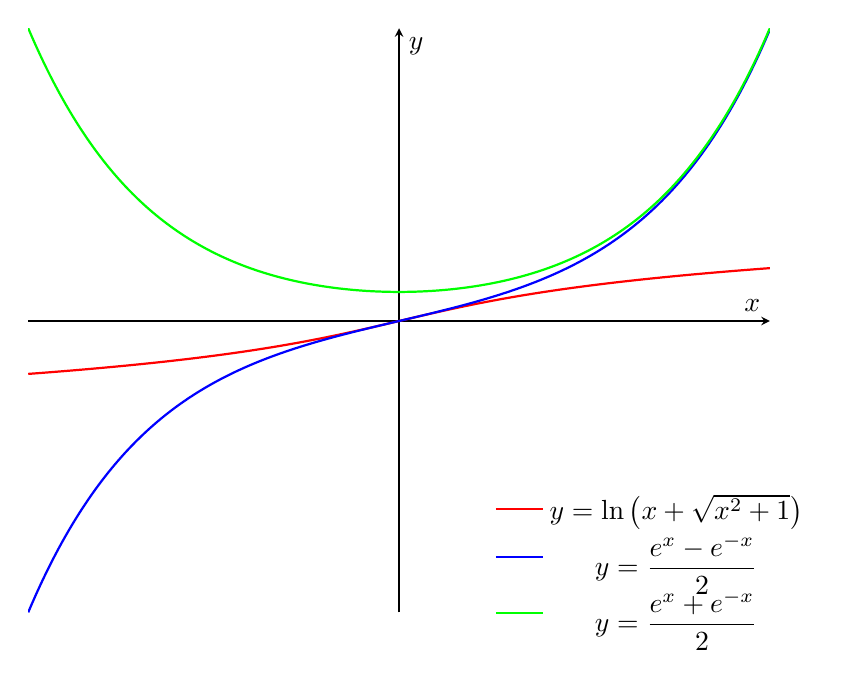
\begin{tikzpicture}
            \begin{axis}
                [
                xshift = -1.8cm,
                axis lines = middle,
                xlabel = {$x$},
                ylabel = {$y$},
                domain = -3:3,
                samples = 200,
                width = 11cm,
                height = 9cm,
                xtick = \empty,
                ytick = \empty,
                legend style={
                    at={(0.02,0.98)},
                    anchor=north west,
                    xshift=160pt,
                    yshift=-160pt,
                    draw=none
                }
                ]

                \addplot[red, thick] {ln(x + sqrt(x^2 + 1))};
                \addlegendentry{$y=\ln\left(x + \sqrt{x^2 + 1}\right)$}

                \addplot[blue, thick] {sinh(x)};
                \addlegendentry{$\displaystyle y=\frac{e^x - e^{-x}}{2}$}

                \addplot[green, thick] {cosh(x)};
                \addlegendentry{$\displaystyle y=\frac{e^x + e^{-x}}{2}$}

            \end{axis}
        \end{tikzpicture}
        \item 函数奇偶性
        \begin{itemize}
            \item $f(x) + f(-x)$必是偶函数
            \item $f(x) - f(-x)$必是奇函数
            \item 任意定义在关于原点对称区间上的函数,
            都可以表示为一个奇函数与一个偶函数之和。

            对任一函数 $f(x)$,定义
            \[
                u(x) = \frac{1}{2}\bigl[f(x) + f(-x)\bigr], \qquad
                v(x) = \frac{1}{2}\bigl[f(x) - f(-x)\bigr].
            \]

            则有 $u(x)$ 是偶函数,$v(x)$ 是奇函数。并且
            \[
                f(x)
                = \frac{1}{2}\bigl[f(x) + f(-x)\bigr]
                + \frac{1}{2}\bigl[f(x) - f(-x)\bigr]
                = u(x) + v(x).
            \]
            \item $f[\psi(x)]$内偶则偶,内奇同外
            \item $\color{red}{\bigstar}$求导一次,奇偶性互换
            \item 设对任意的$x, y$,都有$f(x + y) = f(x) + f(y)$,则$f(x)$是奇函数
        \end{itemize}
        \item 反正弦函数 $y=\arcsin x$ 是函数
        \[
            y=\sin x \quad \left(x\in\left[-\frac{\pi}{2},\,\frac{\pi}{2}\right]\right)
        \]
        的反函数,其主值区间为
        \[
            \arcsin x \in \left[-\frac{\pi}{2},\,\frac{\pi}{2}\right].
        \]
        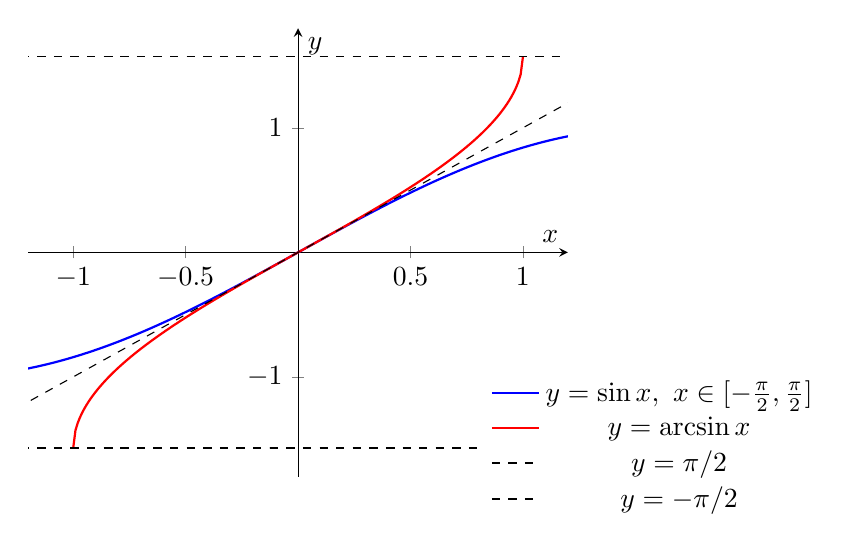
\begin{tikzpicture}
            \begin{axis}
                [
                axis lines = middle,
                xlabel = {$x$},
                ylabel = {$y$},
                xmin = -1.2, xmax = 1.2,
                ymin = -1.8, ymax = 1.8,
                samples = 200,
                legend style={
                    draw=none, at={(0.02,0.98)}, anchor=north west,
                    xshift=160pt,
                    yshift=-120pt,
                }]

% y = sin x (restricted)
                \addplot[blue, thick, domain=-pi/2:pi/2]
                {sin(deg(x))};
                \addlegendentry{$y=\sin x,\ x\in[-\frac{\pi}{2},\frac{\pi}{2}]$}

% y = arcsin x  ← 关键修正
                \addplot[red, thick, domain=-1:1]
                {asin(x)*pi/180};
                \addlegendentry{$y=\arcsin x$}

% y = x
                \addplot[dashed] {x};

                % y = \pi/2
                \addplot[dashed] {1.570796};
                \addlegendentry{$y=\pi/2$}

                % y = -\pi/2
                \addplot[dashed] {-1.570796};
                \addlegendentry{$y=-\pi/2$}
            \end{axis}
        \end{tikzpicture}
        \item 若 $y = \sin x,\ x \in \left(\displaystyle \frac{\pi}{2}, \frac{3\pi}{2}\right)$,则$x = \pi - \arcsin y$
        \item 反余弦函数 $y=\arccos x$ 是函数
        \[
            y=\cos x \quad (x\in[0,\pi])
        \]
        的反函数,其主值区间为
        \[
            \arccos x \in [0,\pi].
        \]
        \begin{tikzpicture}
            \begin{axis}
                [
                axis lines = middle,
                xlabel = {$x$},
                ylabel = {$y$},
                xmin = -1.2, xmax = 1.2,
                ymin = -0.2, ymax = 3.4,
                samples = 200,
                legend style={draw=none, at={(0.02,0.98)}, anchor=north west,xshift=160pt}
                ]

% y = arccos x  ← 关键修正
                \addplot[red, thick, domain=-1:1]
                {acos(x)*pi/180};
                \addlegendentry{$y=\arccos x$}

            \end{axis}
        \end{tikzpicture}

    \end{enumerate}

    \subsection{结论}

    \begin{enumerate}
        \item 当$x \to 0$时,常用的等价无穷小
        \begin{itemize}
            \item $x \sim y = \ln\left(x + \sqrt{x^2 + 1}\right)$
            \item $x \sim \sin x$
            \item $x \sim \tan x$
        \end{itemize}
        \item $x-[x]$是$x$的小数部分,是以1位周期的函数
    \end{enumerate}

    \subsection{定理}

    \begin{enumerate}
    \end{enumerate}

    \subsection{运算}

    \begin{enumerate}

    \end{enumerate}

    \subsection{公式}

    \begin{enumerate}
        \item $\displaystyle x^2 + \frac{1}{x^2} = (x + \frac{1}{x})^2 - 2$
        \item
        \[
            e^x = \sum_{n=0}^{\infty} \frac{x^n}{n!}.
        \]

        广义化:
        \[
            2^x = e^{x\ln 2}
            = \sum_{n=0}^{\infty} \frac{(x\ln 2)^n}{n!}.
        \]
        \item $[x + n] = [x] + n$.
        特别地,当 $n=1$ 时,$[x + 1] = [x] + 1$
    \end{enumerate}

    \subsection{方法步骤}

    \begin{enumerate}

    \end{enumerate}

    \subsection{条件转换思路}

    \begin{enumerate}

    \end{enumerate}

    \subsection{理解}

    \begin{enumerate}
    \end{enumerate}

\end{document}
